\usetikzlibrary{arrows.meta}
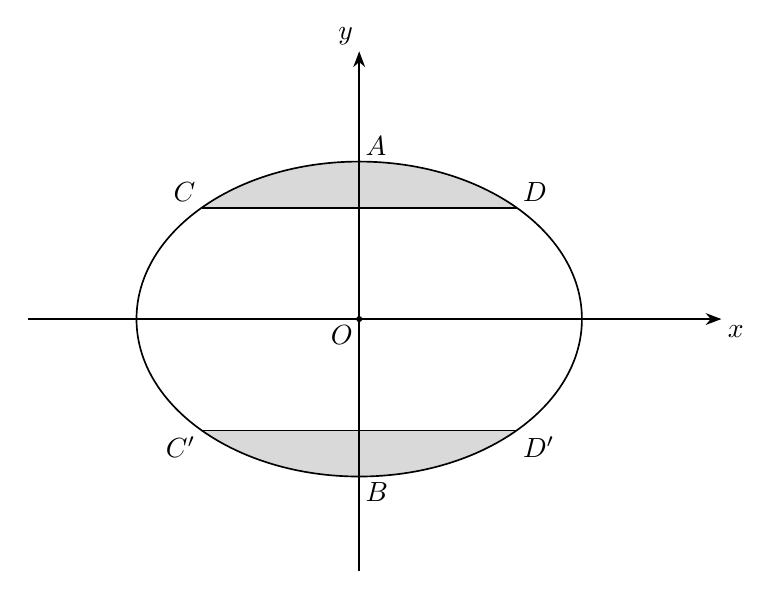
\begin{tikzpicture}[x=1cm,y=1cm,line width=.6pt,font=\normalsize,>=Stealth]
\coordinate (O) at (0,0);
\coordinate (A) at (0,2);
\coordinate (B) at (0,-2);
\coordinate (C) at (-2,1.414213562373);
\coordinate (D) at (2,1.414213562373);
\coordinate (Cp) at (-2,-1.414213562373);
\coordinate (Dp) at (2,-1.414213562373);
\fill[gray!30] (D) arc[start angle=45,end angle=135,x radius=2.828427124746cm,y radius=2cm] -- cycle;
\fill[gray!30] (Cp) arc[start angle=225,end angle=315,x radius=2.828427124746cm,y radius=2cm] -- cycle;
\draw (O) ellipse[x radius=2.828427124746cm,y radius=2cm];
\draw (C) -- (D);
\draw (Cp) -- (Dp);
\draw[->] (-4.2,0) -- (4.6,0) node[below right,inner sep=0pt,xshift=2pt,yshift=-2pt] {$x$};
\draw[->] (0,-3.2) -- (0,3.4) node[above left,inner sep=0pt,xshift=-2pt,yshift=2pt] {$y$};
\fill (O) circle[radius=1.1pt];
\node[below left,inner sep=0pt,xshift=-2pt,yshift=-2pt] at (O) {$O$};
\node[above right,inner sep=0pt,xshift=2pt,yshift=2pt] at (A) {$A$};
\node[below right,inner sep=0pt,xshift=2pt,yshift=-2pt] at (B) {$B$};
\node[above left,inner sep=0pt,xshift=-2pt,yshift=2pt] at (C) {$C$};
\node[above right,inner sep=0pt,xshift=2pt,yshift=2pt] at (D) {$D$};
\node[below left,inner sep=0pt,xshift=-2pt,yshift=-2pt] at (Cp) {$C'$};
\node[below right,inner sep=0pt,xshift=2pt,yshift=-2pt] at (Dp) {$D'$};
\end{tikzpicture}
